\section{Descargas}
El siguiente proyecto con sus respectivos archivos se encuentra para realizar la descarga en el repositorio GITHUB.
poner la tarjeta como imagen
\url{https://opengraph.githubassets.com/1/UNPSJB-YC/Automatizacion_Tunel_UNPSJB}

\url{https://github.com/UNPSJB-YC/Automatizacion_Tunel_UNPSJB}
\newpage
\section{Manual de usuario de la aplicación}
\subsection{Requerimientos del sistema}
\begin{itemize}
	\item Windows
	\item Driver de comunicación serial para CH340 \url{https://electrocrea.com/blogs/tutoriales/como-instalar-driver-ch340-para-arduinos-genericos}
\end{itemize}


\subsection{Puesta en marcha}
\begin{enumerate}
	\item Alimente variador de velocidad y el motor.
	\item Enchufe a 220V el cable de alimentación que sale de la implementación física.
	\item Conecte el cable serial USB que sale de la implementación física.
	\item Ejecute el programa \fcolorbox{red}{yellow}{“NOMBRE.EXE”}
	\item Seleccione el puerto dónde se encuentra conectado el microcontrolador.
	\item Active el puerto.
	\item Al inicializar el puerto, el microcontrolador comienza a entregar valores a la aplicación por lo que se observa THP, velocidad estimada y frecuencia de referencia. 
	
\end{enumerate}

\begin{figure}[H]
	\centering
	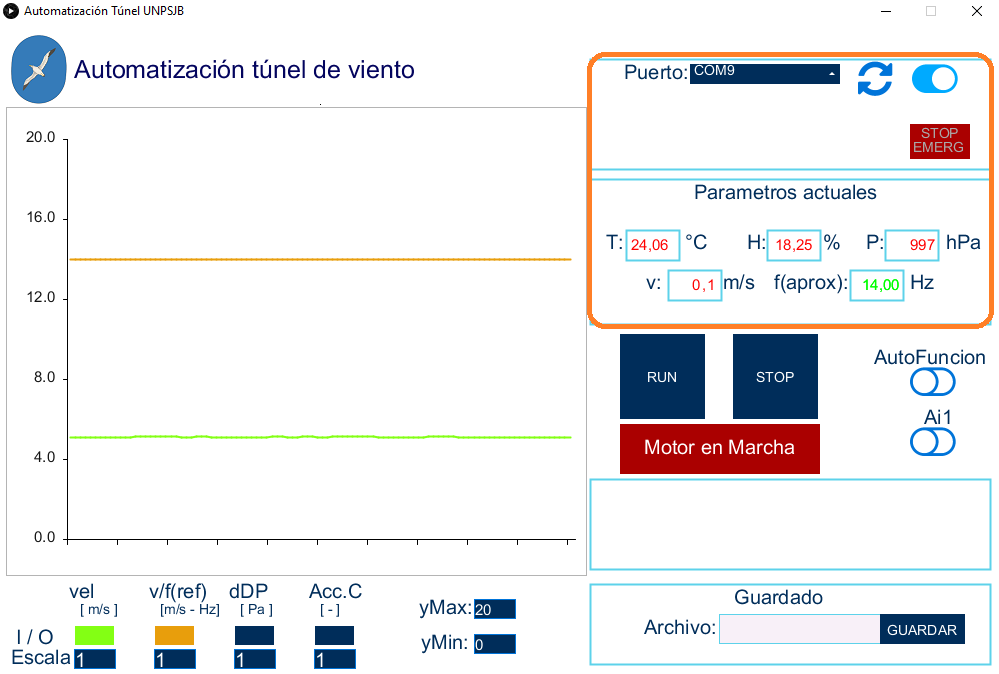
\includegraphics[scale=0.5]{capt2.png}
	\captionof{figure}{Puerto activado. Visualización de los valores del $\mu$C.}
	\label{fig:capt2}
\end{figure}



\subsection{Gráfico en tiempo real}
\subsubsection{	Visibilidad de las señales en tiempo real}
En la parte izquierda inferior del programa, se puede activar o desactivar la visibilidad de las variables a observar en tiempo real, solo basta realizar un click en los rectángulos, y estos al estar activados se colocarán del color correspondiente a la señal a observar.

\subsubsection{Escala}
En la parte inferior se encontrará “Escala” donde se establece la escala correspondiente de cada señal.
\begin{enumerate}
	\item Realice click en el interior del rectángulo
	\item Borre el número que posee y colocar el valor nuevo a ingresar.
	\item Presione “enter”.
	\item La escala de la señal elegida será modificada.
	
\end{enumerate}

\textbf{Ejemplo de escala:}

Si se coloca en una señal “10”, la variable observada en tiempo real estará aumentada 10 veces.

\subsubsection{Límite del eje vertical}
El eje vertical del gráfico en tiempo real puede ser modificado según necesidad.

\begin{enumerate}
	\item Realice click en el interior del rectángulo.
	\item Borre el número que posee y colocar el valor nuevo a ingresar.
	\item Presione “enter”.
	\item El eje “vertical” se verá modificado.
	
\end{enumerate}


\begin{figure}[H]
	\centering
	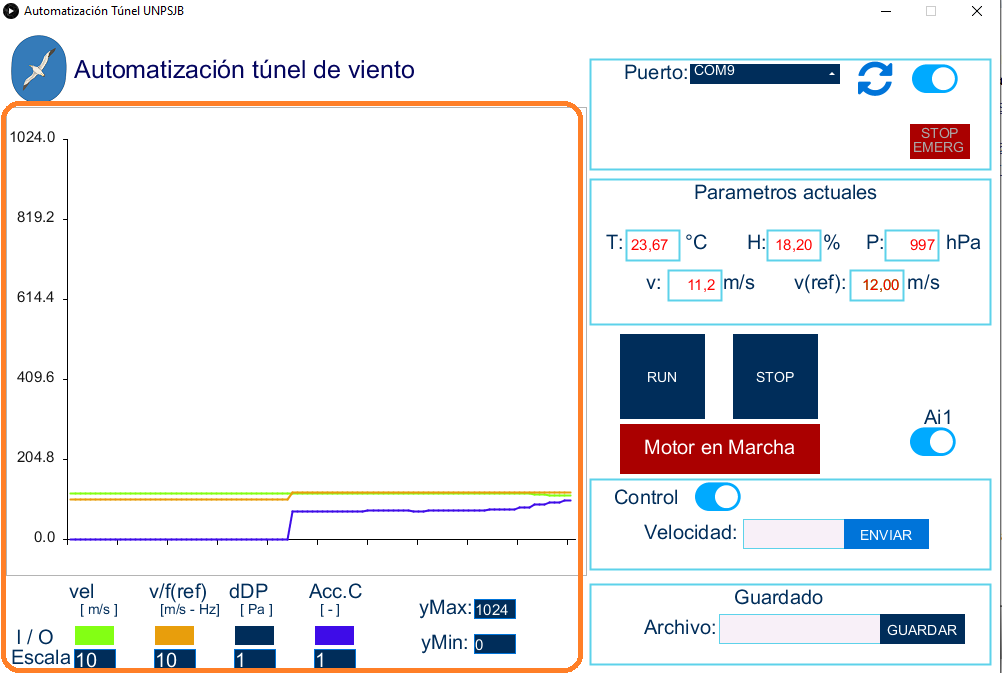
\includegraphics[scale=0.5]{capt3.png}
	\captionof{figure}{Gráfico en tiempo real}
	\label{fig:capt3}
\end{figure}

\subsection{AutoFuncion}
El modo de auto-función carga un archivo “.csv” que se encuentra dentro de la carpeta “autofun”. El archivo “.csv” posee los datos pertenecientes a los escalones de velocidad deseados y el tiempo de ejecución de cada uno.

\begin{figure}[htb]
	\centering
	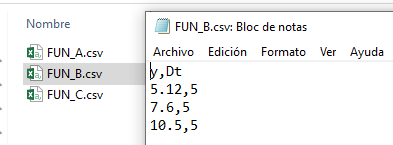
\includegraphics[scale=0.7]{carpcsv.png}
	\captionof{figure}{Archivos dentro de la carpeta "{}autofun"}
	\label{fig:autof2}
\end{figure}


El archivo tiene que tener el formato observado en la Tabla \ref{tab:formcsv}, donde se ve que posee un encabezado. Si se desea que la velocidad sea un número decimal, este debe ir con punto. 
\begin{table}[h]
	\centering
	\begin{tabular}{|l|}
		\hline
		y,Dt \\ \hline
		y1,Dt1 \\ \hline
		y2,Dt2 \\ \hline
		y3,Dt3 \\ \hline
	\end{tabular}
	
	\caption{Formato .csv}
	\label{tab:formcsv}
\end{table}

Mientras que se ejecute esta función aparecerá una señal visual debajo del botón abrir. (Figura \ref{fig:autof1})

\begin{figure}[htb]
	\centering
	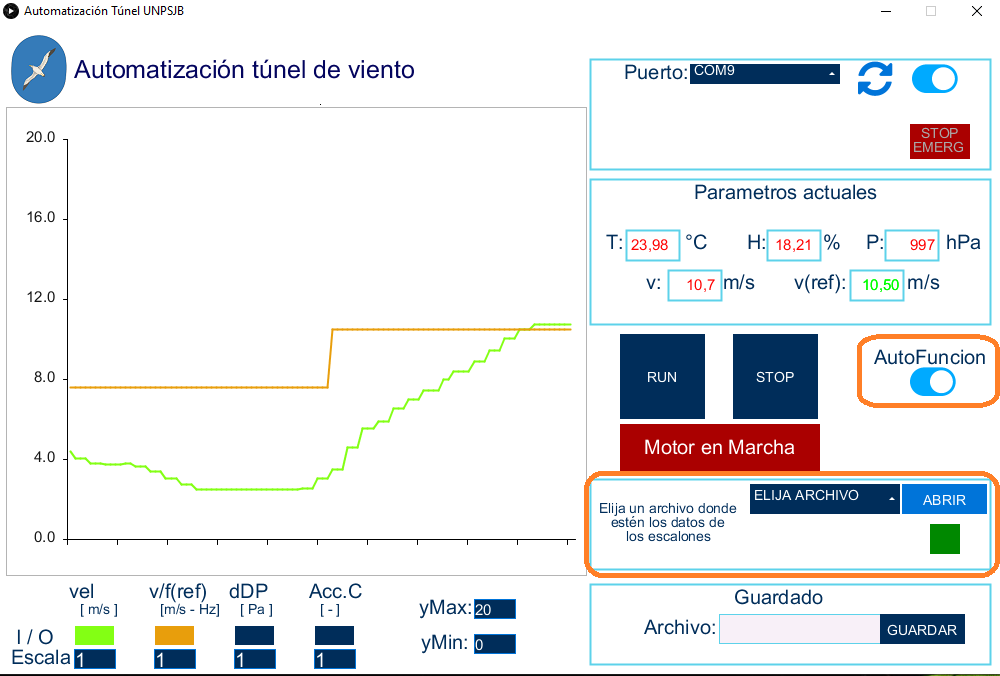
\includegraphics[scale=0.5]{capt1.png}
	\captionof{figure}{Aplicación en modo Autofunción}
	\label{fig:autof1}
\end{figure}



\subsection{Ai1}
\subsubsection{Control desactivado}
Al utilizar este modo de funcionamiento, se puede ingresar un valor aproximado de frecuencia. El lazo de control estará abierto.

\subsubsection{Control activado}
El lazo de control estará activado, ante perturbaciones el sistema tiende a establecerse a la velocidad estipulada. Para estipular la velocidad se debe presionar sobre la caja de “velocidad” ingresar un valor y presionar sobre el botón “enviar”.

\subsection{Encendido/ apagado del motor}
El encendido/ apagado del motor se puede realizar de dos formas:
\subsubsection{Panel frontal}
Si el parámetro F7 del variado de velocidad se encuentra en “0”, la marcha y parada del motor será realizada por los botones físicos el panel frontal.
\subsubsection{Aplicación}
Si el parámetro F7 del variador de velocidad se encuentra en “1”, la marcha y parada del motor será realizada por los botones propios de la aplicación.


\subsection{Guardado de datos}
Al colocar un nombre y presionar el botón guardar, se generará un archivo “.csv” con los datos que el microcontrolador capturó cada aproximadamente 55ms. Estos archivos se guardarán en la carpeta "data1" en la carpeta general de la aplicación. 

\textbf{\textit{Alerta:}} Una vez que se presiona el botón guardar o el puerto se cierra los datos son borrados y se comenzará una nueva tabla.

\begin{figure}[H]
	\centering
	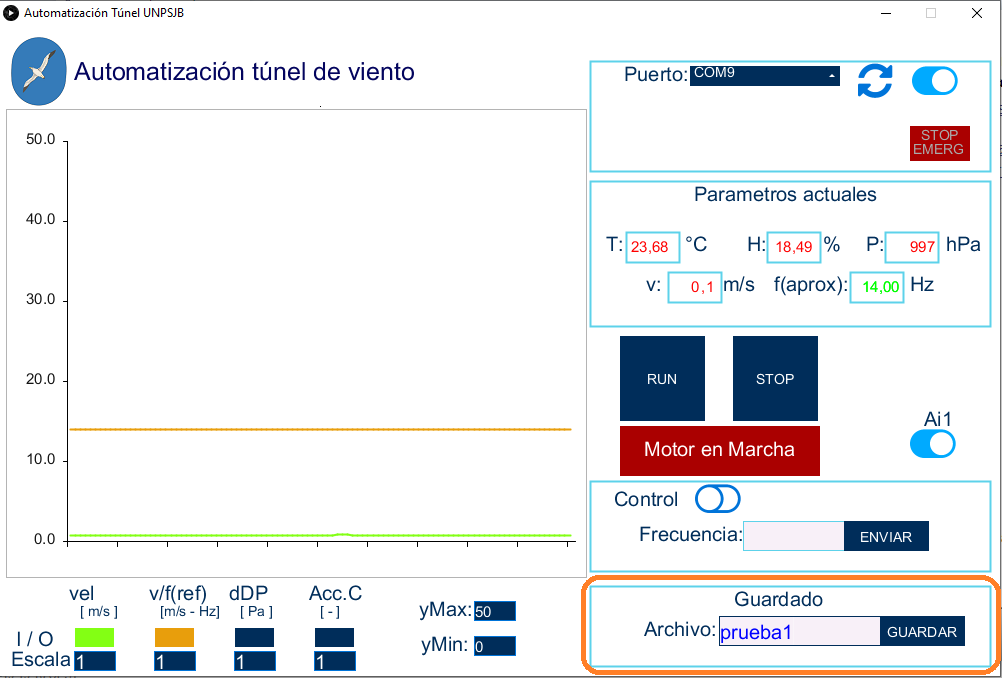
\includegraphics[scale=0.5]{capt4.png}
	\captionof{figure}{Guardado de datos}
	\label{fig:capt4}
\end{figure}


\subsection{Lectura de datos obtenidos}
El encabezado de la tabla (Figura \ref{fig:capt5}) muestra las siguientes leyendas:

\begin{itemize}
	\item \textit{Muestra:} número de muestra tomada
	\item \textit{Tiempo:} tiempo desde el inicio del puerto serie [ms].
	\item \textit{Temp:} temperatura ambiente [$^{\circ}$ C].
	\item \textit{Hum:} humedad relativa del ambiente [\%].
	\item \textit{Pres:} presión atmosférica [hPa].
	\item \textit{Den:} densidad estimada por el microcontrolador [$kg/m^3$].
	\item \textit{DP:} diferencia de presión medida a través del MPX7002 en conjunto con ADS1115 [Pa]
	\item \textit{Ref:} Valor de frecuencia o velocidad preestablecida [Hz ó m/s].
	\item \textit{VelFrec:} Velocidad del aire estimada [m/s].
	\item \textit{PWM:} señal de acción de control.
	\item \textit{Control:} señal de que el lazo de control está cerrado.
	\item \textit{Error:} error entre la velocidad estimada y la de referencia.
	\item \textit{ESTADOvariador:} estado encendido/apagado del motor.
	\item \textit{ERRORvariador:} indicación de algún error del variador de velocidad.
	\item \textit{TiempoRel:} indica tiempo desde el ultimo guardado de datos.
	\item \textit{ControlAutomatico:} indicación de comienzo y fin del control automático.
		
\end{itemize}

Para hacer lectura o interpretación de los datos se recomienda utilizar el script de matlab \fcolorbox{red}{yellow}{“NOMBRE DEL ARCHIVO DE MATLAB”}

\begin{figure}[H]
	\centering
	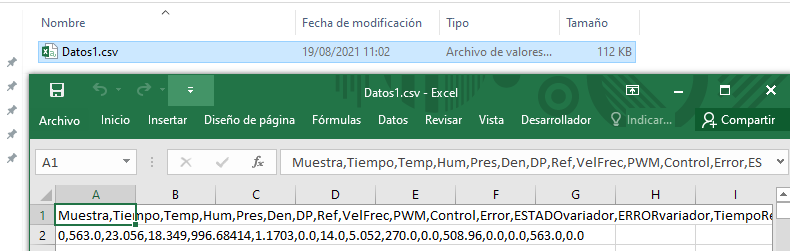
\includegraphics[scale=0.5]{capt5.png}
	\captionof{figure}{Archivo .csv generado}
	\label{fig:capt5}
\end{figure}

\subsection{Falla externa}
	Al presionar el botón de “Falla externa” el $\mu$C enviará una señal al variador y el sistema se detendrá.

\newpage
\section{Código Arduino}
\newpage
\section{Código Processing}
\newpage
\section{Código Matlab}

